\chapter{Verification \& Validation}
\label{chap:v_and_v}
\graphicspath{{V&V/}}

In this chapter, we will present the results on verification and validation of the simulator discussed in \Cref{chap:naos}. We verify the gravity model, the launch conditions for the regolith, the numerical integrator along with the equations of motion for the regolith, and finally the Solar perturbation models. We validate our simulator to ensure that our inferences for any scientific result out of it remains true and valid as well.

\section{Constant Density Ellipsoid Gravity Model}
\label{sec:gravity_vv}
The \gls{CDE} gravity model was tested for a singular target point by comparing the gravitational potential and acceleration values at that point as computed by \gls{NAOS}, with external data obtained from another researcher at CSML \footnote{Centre for Spaceflight Mechanics Laboratory; The thesis work was partly done at CSML, which is a research lab headed by Dr. Daniel Scheeres and is part of the University of Colorado, Boulder, USA.}. The parameters used for the test are given in \Cref{tab:gravity_vv_params}.
%%%
\begin{table}[htb]
\centering
\captionsetup{justification=centering}
\caption{Parametric values used for testing the \gls{CDE} gravitational potential model.}
\label{tab:gravity_vv_params}
\begin{tabular}{|l|l|l|}
\hline
\multicolumn{1}{|c|}{\textbf{Parameter}} & \multicolumn{1}{c|}{\textbf{Value}} & \multicolumn{1}{c|}{\textbf{Units}}      \\ \hline
Gravitational Parameter                  & 446382.0                            & \si{\metre \cubed \per \second \squared} \\ \hline
Alpha (longest axis of \gls{CDE})      & 20000                               & \si{\metre}                            \\ \hline
Beta (Intermediate axis of \gls{CDE})  & 7000                                & \si{\metre}                            \\ \hline
Gamma (Shortest axis of \gls{CDE})     & 7000                                & \si{\metre}                            \\ \hline
Target point x-coordinate                & 10000                               & \si{\metre}                            \\ \hline
Target point y-coordinate                & 13000                               & \si{\metre}                            \\ \hline
Target point z-coordinate                & 8000                                & \si{\metre}                            \\ \hline
\end{tabular}
\end{table}
\FloatBarrier
%%%
The test values for the gravitational potential and the acceleration values at the specified target point are given in \Cref{tab:gravity_vv_test_values}.
%%%
% Please add the following required packages to your document preamble:
% \usepackage{multirow}
\begin{table}[htb]
\centering
\captionsetup{justification=centering}
\caption{Test values for verification of the \gls{CDE} gravity model.}
\label{tab:gravity_vv_test_values}
\begin{tabular}{|l|l|l|l|}
\hline
\multicolumn{1}{|c|}{\textbf{Parameter}}    & \multicolumn{2}{c|}{\textbf{Value}}     & \multicolumn{1}{c|}{\textbf{Units}}          \\ \hline
Gravitational Potential                     & \multicolumn{2}{l|}{23.710052554396402} & \si{\metre \squared \per \second \squared} \\ \hline
\multirow{3}{*}{Gravitational Acceleration} & x       & -0.00044762916738340803       & \si{\metre \per \second \squared}          \\ \cline{2-4}
                                            & y       & -0.0009623388813999501        & \si{\metre\per \second \squared}           \\ \cline{2-4}
                                            & z       & -0.000592208542399969         & \si{\metre\per \second \squared}           \\ \hline
\end{tabular}
\end{table}
\FloatBarrier
%%%
The values obtained from the simulator \gls{NAOS} were compared with the ones in \Cref{tab:gravity_vv_test_values} upto the 12th decimal point and they matched, validating the gravity model implemented in \gls{NAOS}.

\section{Regolith Launch Conditions}
\label{sec:regolith_launch_conditions_vv}
In this section, we'll presents results on verifying whether the initial state vector for the regolith or the launch condition match to what is desired by the user. Here, an internal validation is done to ensure that the launch conditions registered in the output database match the raw value input to \gls{NAOS}. We present graphical and numerical results in this regard.

\subsection{Launch Location}
\label{subsec:launch_location_vv}
The position vector to the launch location, from the centre of the \gls{ARF}, is formed by giving only the launch location latitude and longitude as input. Thus, we have to verify whether the position vector conforms to a given angular input. We take the initial state vector, from the output databases of the dynamics simulator, of regolith launched from a few launch locations on the asteroid and convert the Cartesian coordinates back to latitude and longitude to see if the position vector was formed correctly. For the same Cartesian coordinates, we use the triaxial ellipsoid equation, and see if they solve the equation, to verify that the launch point lies on the surface of the asteroid.
%
\newline\newline
%
We took 5 test locations from where regolith was launched and separately calculated the corresponding longitude and latitude for the launch location to check if the position vector was correctly formed. The position coordinates and the back-calculated latitude and longitude angles are shown in \Cref{tab:position_vector_to_lat_long_vv}.
%%%
\begin{table}[htb]
\centering
\captionsetup{justification=centering}
\caption{Position vector to different launch locations and the corresponding Latitude and Longitude angles.}
\label{tab:position_vector_to_lat_long_vv}
\begin{tabular}{|c|c|c|c|c|}
\hline
\textbf{X {[}m{]}} & \textbf{Y {[}m{]}} & \textbf{Z {[}m{]}} & \textbf{Longitude {[}deg{]}} & \textbf{Latitude {[}deg{]}} \\ \hline
20000.0 & 0.0 & 0.0 & 0.0 & 0.0 \\ \hline
0.0 & 7000.0 & 0.0 & 90.0 & 0.0 \\ \hline
0.0 & 0.0 & 7000.0 & 0.0 & 90.0 \\ \hline
3316.14545023 & 1914.57746836 & 6632.29090046 & 30.0 & 60.0 \\ \hline
-3961.38284482 & -3961.38284482 & 5602.2413449 & -135.0 (225.0) & 45.0 \\ \hline
\end{tabular}
\end{table}
\FloatBarrier
%%%
The longitude and latitude values given in \Cref{tab:position_vector_to_lat_long_vv} were calculated from the Cartesian coordinates and match those given as inputs to the dynamics simulator. The position vectors from \Cref{tab:position_vector_to_lat_long_vv} with the \gls{CDE} model are also depicted in \Cref{fig:position_vector_diagram}.
%%%
\begin{figure}[htb]
\centering
\captionsetup{justification=centering}
\subfloat[]{
    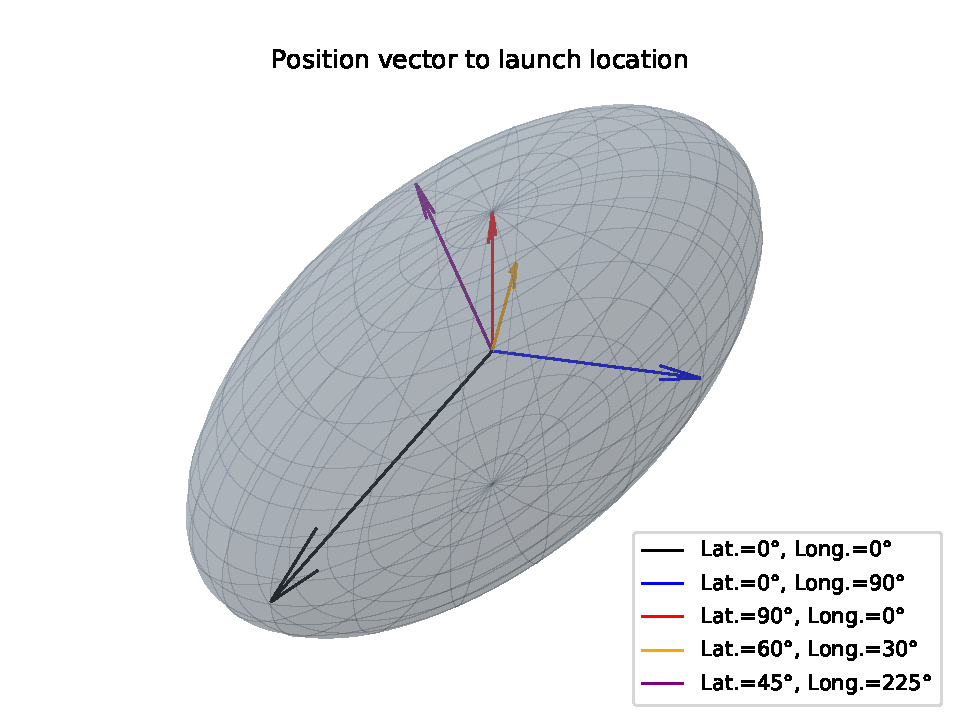
\includegraphics[width=\textwidth, height=0.4\textheight, keepaspectratio=true]{Images/launch_location_position_vectors.pdf}
    \label{fig:launch_location_vv_1}
    }

\subfloat[]{
    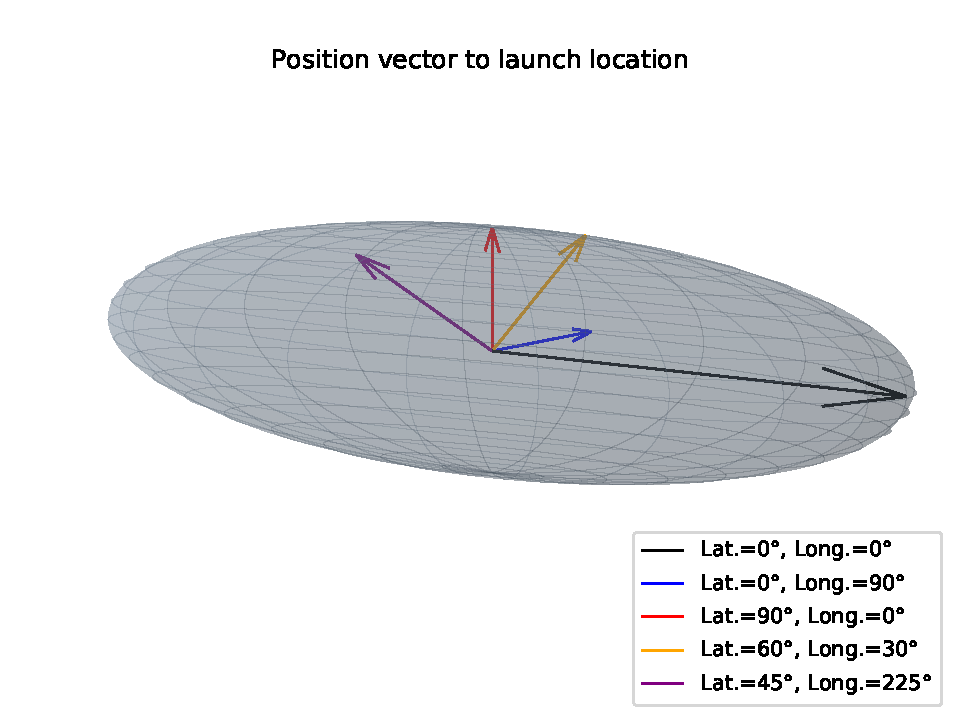
\includegraphics[width=\textwidth, height=0.4\textheight, keepaspectratio=true]{Images/launch_location_position_vectors_2.pdf}
    \label{fig:launch_location_vv_2}
    }
\caption{Position vectors from \protect\Cref{tab:position_vector_to_lat_long_vv} shown with the \protect\gls{CDE} asteroid model.}
\label{fig:position_vector_diagram}
\end{figure}
\FloatBarrier
%%%
We also checked whether the launch location in fact did lie exactly on the surface of the \gls{CDE} asteroid and not inside or above the surface. This is really important because a wrong initial condition could produce erroneous results. Once we substitute the Cartesian coordinates into the triaxial ellipsoid equation (see \Cref{eqn:launch_loc_ellipsoid_eqn_cartesian}) and if the output equals zero (when we take the term 1.0 on the right hand side in \Cref{eqn:launch_loc_ellipsoid_eqn_cartesian}), then the launch point lies on the asteroid. We did an external validation for this but an internal validation always takes place within the dynamics simulator at all times whenever a new simulation is run.
%%%
\begin{table}[htb]
\centering
\captionsetup{justification=centering}
\caption{Output of the triaxial ellipsoid equation for a few test launch location position vectors. An output of 0.0 means that the position vector is a perfect root of the equation and hence the launch location indeed lies on the surface of the asteroid.}
\label{tab:launch_location_surface_vv}
\begin{tabular}{|c|c|c|c|}
\hline
\textbf{X {[}m{]}} & \textbf{Y {[}m{]}} & \textbf{Z {[}m{]}} & \textbf{Output of triaxial ellipsoid equation} \\ \hline
20000.0 & 0.0 & 0.0 & 0.0 \\ \hline
0.0 & 7000.0 & 0.0 & 0.0 \\ \hline
0.0 & 0.0 & 7000.0 & 0.0 \\ \hline
3316.14545023 & 1914.57746836 & 6632.29090046 & 2.22044604925e-16 \\ \hline
-3961.38284482 & -3961.38284482 & 5602.2413449 & 0.0 \\ \hline
\end{tabular}
\end{table}
\FloatBarrier
%%%

\subsection{Launch Velocity}
\label{subsec:launch_velocity_vv}
The launch velocity vector is formed by providing two angles and a magnitude. As explained in \Cref{subsec:launch_velocity}, the two angles are the declination angle from the normal vector at the launch location and the azimuth angle from the local North direction. The local North direction and the normal vector, in essence, act as the basis vectors for a local surface frame of reference which in turn help in the mathematical formulation of the velocity vector of Cartesian components. Since we are dealing with an ellipsoid and not a sphere, defining local North is not a straight-forward process as explained earlier in \Cref{subsec:launch_velocity}.
%
\newline\newline
%
Thus, we first begin with verifying our methodology of forming the local surface frame, and ensure that the local Normal vector and the local North pointing vector are correctly formed and their lies no discrepancy. Then we verify whether the velocity vector, in terms of its Cartesian components, indeed makes the same angle with the surface frame as specified at the input of the simulation. The process for the second verification item is different from how the velocity vector was formed in the first place and hence the verification itself won't be a tampered or faulty process.
%
\newline\newline
%
Let's first begin with a test launch location at the longest edge of the \gls{CDE}. A graphical depiction of the frame is shown in \Cref{fig:surface_frame}. This is the simplest location to perform any simulation or test because the surface normal vector here will be along the same direction as the position vector to the launch point from the centre of the ellipsoid. This also makes the test in itself a trivial task. Note that the surface normal is also the z-axis for the surface frame at the launch point. So for the current test location, if the cross product of the normal and the position vector is a zero vector, then the normal vector is verified. \Cref{tab:longest_edge_surface_frame_vv} shows the result for this. Following this, if the angle between the normal vector and the x-axis basis vector for the surface frame is \SI{90}{\degree}, then the latter is pointing to the local North direction. This is because for the current test location, any vector perpendicular to the surface normal (or effectively to the launch location position vector) will be along the \SI{0}{\degree} meridian line crossing the test location. A simple dot product (again shown in \Cref{tab:longest_edge_surface_frame_vv}) between the x-axis basis vector of the surface frame and the normal vector will tell us if they are perpendicular to each other or not.
%%%
\begin{table}[htb]
\centering
\captionsetup{justification=centering}
\caption{Surface frame verification at the longest edge of the ellipsoid}
\label{tab:longest_edge_surface_frame_vv}
\begin{tabular}{|l|l|l|l|c|}
\hline
\multicolumn{1}{|c|}{\textbf{Unit Vector}} & \multicolumn{3}{c|}{\textbf{Components}} & \textbf{Operations} \\ \hline
\multicolumn{1}{|c|}{} & \multicolumn{1}{c|}{x} & \multicolumn{1}{c|}{y} & \multicolumn{1}{c|}{z} & \multicolumn{1}{l|}{} \\ \hline
Position ($\buv{r}$) & 1.0 & 0.0 & 0.0 & \multirow{2}{*}{$\buv{r} \times \buv{n}$ = {[}0.0, 0.0, 0.0{]}} \\ \cline{1-4}
Normal ($\buv{n}$) & 1.0 & 0.0 & 0.0 &  \\ \hline
X-axis Surface frame / local North direction ($\buv{x}$) & 0.0 & 0.0 & 1.0 & \multicolumn{1}{l|}{$\buv{x} \cdotp \buv{n}$ = 0.0} \\ \hline
\end{tabular}
\end{table}
\FloatBarrier
%%%
Now, we perform a more generalized and non-trivial test for the surface frame but this time we choose a more general launch location. A test site was chosen at \SI{30}{\degree} longitude and \SI{60}{\degree} latitude. It can be viewed in \Cref{fig:surface_frame_leadingEdge_vv}. Note that at this location, the surface normal vector and the launch position vector will not be aligned. We begin with first verifying that the x-axis basis vector for the surface frame at the current launch site is pointing to North. Another way of stating this is that this vector is tangential to the meridian line, which is running all the way up to the poles. If the x-axis basis vector is indeed tangential to the local meridian, then its x-y plane projection will be collinear to that of the position vector to the launch site.
%%%
\begin{table}[htb]
\begin{adjustwidth}{-1in}{-1in}
\centering
\captionsetup{justification=centering}
\caption{Surface frame verification for test launch location at \SI{30}{\degree} Longitude and \SI{60}{\degree} Latitude, i.e., on the leading edge of the asteroid.}
\label{tab:leading_edge_surface_frame_vv}
\begin{tabular}{|l|c|c|c|c|}
\hline
\multicolumn{1}{|c|}{\textbf{Unit Vector}} & \multicolumn{3}{c|}{\textbf{Components}} & \textbf{Operations} \\ \hline
\multicolumn{1}{|c|}{} & x & y & z & \multicolumn{1}{l|}{} \\ \hline
Position ($\buv{r}$) & 0.4330127 & 0.25 & 0.8660254 & \multirow{2}{*}{\begin{tabular}[c]{@{}c@{}}$\buv{x}_x / \buv{r}_x == \buv{x}_y / \buv{r}_y$ \\ = -1.9621431353\end{tabular}} \\ \cline{1-4}
X-axis Surface frame / local North direction ($\buv{x}$) & -0.8496329 & -0.49053578 & 0.1936455 &  \\ \hline
Normal ($\buv{n}$) & 0.05874547 & 0.27687111 & 0.95910967 & \multicolumn{1}{l|}{$\buv{n} \cdotp \buv{x} = 0.0$} \\ \hline
\end{tabular}
\end{adjustwidth}
\end{table}
\FloatBarrier
%%%
%%%
\begin{figure}[htb]
\centering
\captionsetup{justification=centering}
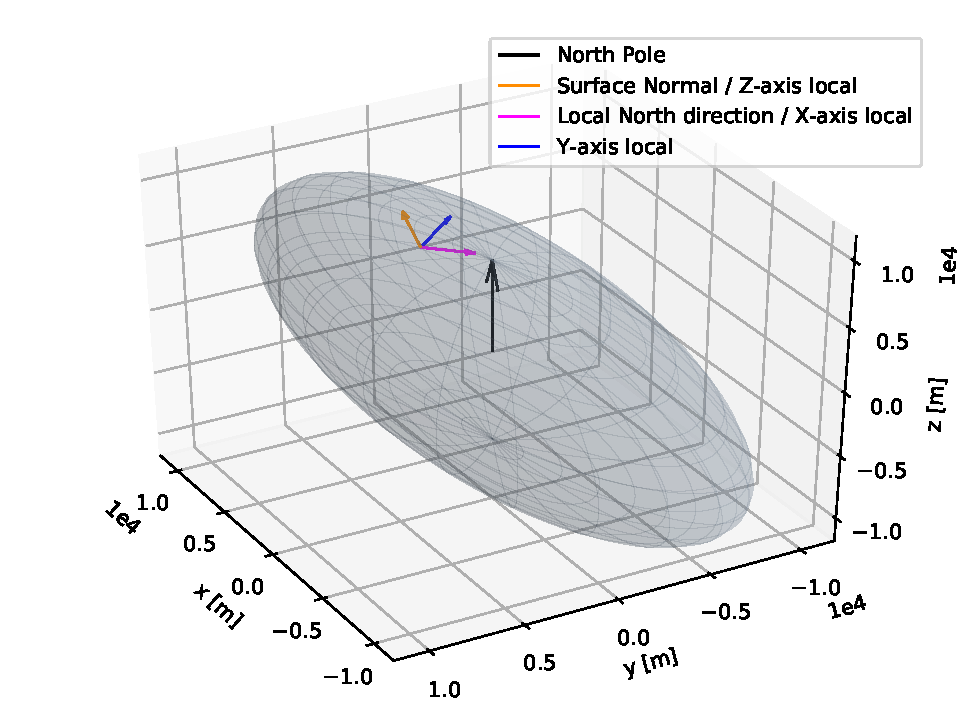
\includegraphics[width=\textwidth, height=0.35\textheight, keepaspectratio=true]{Images/surface_frame_leadingEdge.pdf}
\caption{Surface frame depicted for test launch located at \SI{30}{\degree} Longitude and \SI{60}{\degree} Latitude. Note that the longitude is measured in anti-clockwise direction from the +X axis in the figure.}
\label{fig:surface_frame_leadingEdge_vv}
\end{figure}
\FloatBarrier
%%%
We can prove the two projections to be collinear if the x and the y components of the vectors form equal ratios. This is shown in \Cref{tab:leading_edge_surface_frame_vv}. We see that the ratios are equal and hence the x-axis basis vector is pointing to the North direction. Following this, we can also say that the normal vector at this location is formulated correctly since it is perpendicular to the x-axis basis vector (which in turn is tangential to the meridian line). A vector perpendicular to the meridian line will in-fact be the surface normal vector. Note that, we haven't explicitly verified the y-axis basis vector of the surface frame because it is formed by cross multiplying the normal and the x-axis basis vector. So it inherently remains verified if the latter two are formulated correctly.
%
\newline\newline
%
Now that we have verified that the surface frame is established correctly, we need to verify that the velocity vector makes the correct declination and azimuth angle with the surface frame. The test launch location is still the same as before and the procedure for verification (explained shortly) is different from how the velocity vector was originally formed. We use the vector dot product definition to compute the angle between the velocity vector and the surface normal vector. This gives us the launch declination angle. We then compute the projection of the velocity vector onto the x-y plane of the surface frame \footnote{Given a velocity vector \bvt{v} and the surface normal vector \bvt{n}, the x-y plane projection of \bvt{v} is given as: $\bv{v}_{xy} = \bv{v} - \frac{\bv{v} \cdotp \bv{n}}{n^2} \bv{n}$} and then compute the angle between the projection and the x-axis basis vector of the surface frame. The latter is done, again, by using the dot product method. This then gives us the launch azimuth angle. If the computed angles match the ones provided as input for the simulation, then the velocity vector formulation is verified.
%
\newline\newline
%
Two particle launches were simulated for the aforementioned verification process. The particles were launched with a velocity of 6.0 [m/s] from a point located on the surface of the \gls{CDE} asteroid at \SI{30}{\degree} Longitude and \SI{60}{\degree} Latitude. The first test involved launching particles at declination and azimuth angles of \SI{30}{\degree} and \SI{45}{\degree} respectively. The second test involved declination and azimuth angles of \SI{60}{\degree} and \SI{135}{\degree} respectively. The results for these test simulations is shown in \Cref{tab:launch_velocity_angle_vv_1,tab:launch_velocity_angle_vv_2}. \Cref{fig:launch_velocity_angles_vv} shows the orientation of the velocity vector, for the first test, with respect to the launch site surface frame and the \gls{ARF}.
%%%
\begin{table}[htb]
\begin{adjustwidth}{-1in}{-1in}
\centering
\captionsetup{justification=centering}
\caption{Launch velocity surface frame angles verification data. Input launch declination = \SI{30}{\degree} and azimuth = \SI{45}{\degree}.}
\label{tab:launch_velocity_angle_vv_1}
\begin{tabular}{|l|c|c|c|c|c|}
\hline
\multicolumn{1}{|c|}{\textbf{Vector}} & \multicolumn{3}{c|}{\textbf{\begin{tabular}[c]{@{}c@{}}Vector\\ Components\end{tabular}}} & \textbf{\begin{tabular}[c]{@{}c@{}}Launch\\ Declination {[}deg{]}\end{tabular}} & \textbf{\begin{tabular}[c]{@{}c@{}}Launch\\ Azimuth {[}Deg{]}\end{tabular}} \\ \hline
\multicolumn{1}{|c|}{} & x & y & z &  &  \\ \hline
Velocity ($\bv{v}$) {[}m/s{]} & -0.385325 & -1.354695 & 5.832351 &  & \multicolumn{1}{l|}{\cellcolor[HTML]{9B9B9B}} \\ \cline{1-4}
Unit Normal & 0.058745 & 0.276871 & 0.959109 & \multirow{-2}{*}{30.0} & \multicolumn{1}{l|}{\multirow{-2}{*}{\cellcolor[HTML]{9B9B9B}}} \\ \hline
$\bv{v}$ projection {[}m/s{]} & -0.690575 & -2.793360 & 0.848671 & \multicolumn{1}{l|}{\cellcolor[HTML]{9B9B9B}} &  \\ \cline{1-4}
Unit x-axis surface frame & -0.8496329 & -0.49053578 & 0.1936455 & \multicolumn{1}{l|}{\multirow{-2}{*}{\cellcolor[HTML]{9B9B9B}}} & \multirow{-2}{*}{45.0} \\ \hline
\end{tabular}
\end{adjustwidth}
\end{table}
\FloatBarrier
%%%
%%%
\begin{table}[htb]
\begin{adjustwidth}{-1in}{-1in}
\centering
\captionsetup{justification=centering}
\caption{Launch velocity surface frame angles verification data. Input launch declination = \SI{60}{\degree} and azimuth = \SI{135}{\degree}.}
\label{tab:launch_velocity_angle_vv_2}
\begin{tabular}{|l|c|c|c|c|c|}
\hline
\multicolumn{1}{|c|}{\textbf{Vector}} & \multicolumn{3}{c|}{\textbf{\begin{tabular}[c]{@{}c@{}}Vector\\ Components\end{tabular}}} & \textbf{\begin{tabular}[c]{@{}c@{}}Launch\\ Declination {[}deg{]}\end{tabular}} & \textbf{\begin{tabular}[c]{@{}c@{}}Launch\\ Azimuth {[}Deg{]}\end{tabular}} \\ \hline
\multicolumn{1}{|c|}{} & x & y & z &  &  \\ \hline
Velocity ($\bv{v}$) {[}m/s{]} & 5.223625 & -0.4029416 & 2.924273 &  & \multicolumn{1}{l|}{\cellcolor[HTML]{9B9B9B}} \\ \cline{1-4}
Unit Normal & 0.058745 & 0.276871 & 0.959109 & \multirow{-2}{*}{60.0} & \multicolumn{1}{l|}{\multirow{-2}{*}{\cellcolor[HTML]{9B9B9B}}} \\ \hline
$\bv{v}$ projection {[}m/s{]} & 5.047389 & -1.2335549 & 0.046944 & \multicolumn{1}{l|}{\cellcolor[HTML]{9B9B9B}} &  \\ \cline{1-4}
Unit x-axis surface frame & -0.8496329 & -0.4905357 & 0.1936455 & \multicolumn{1}{l|}{\multirow{-2}{*}{\cellcolor[HTML]{9B9B9B}}} & \multirow{-2}{*}{135.0} \\ \hline
\end{tabular}
\end{adjustwidth}
\end{table}
\FloatBarrier
%%%
%%%
\begin{figure}[htb]
\centering
\captionsetup{justification=centering}
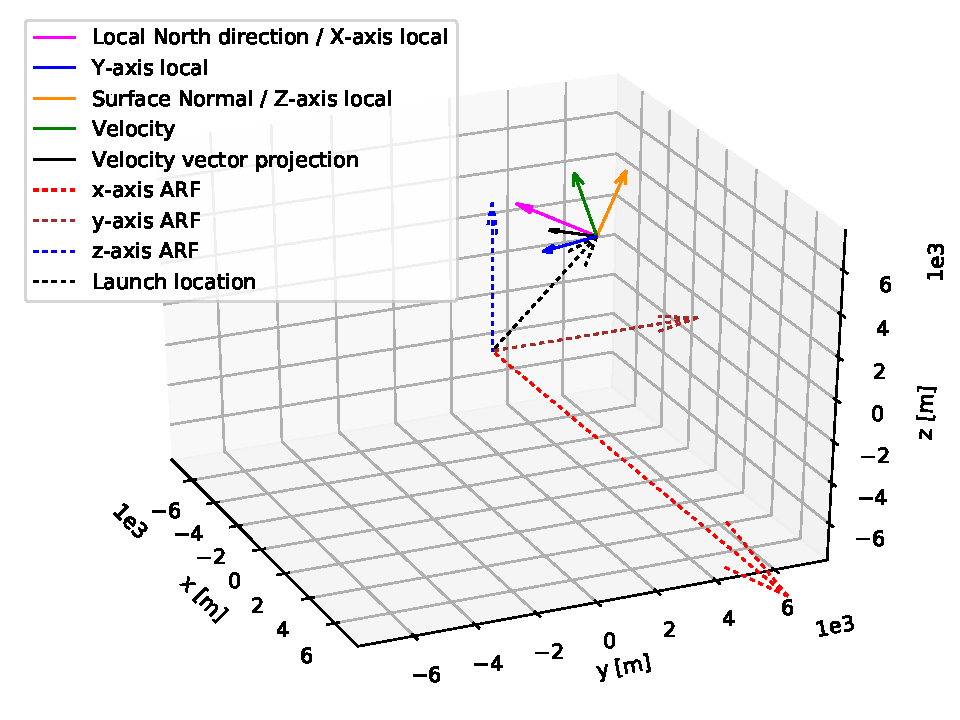
\includegraphics[width=\textwidth, height=0.6\textheight, keepaspectratio=true]{Images/velocity_vector_angles_vv.pdf}
\caption{Schematic representing the surface frame for launch site at \SI{30}{\degree} Longitude and \SI{60}{\degree} Latitude along with the velocity vector and the \gls{ARF}. The diagram gives an intuition on the orientation of the velocity vector. The launch declination and azimuth angles are \SI{30}{\degree} and \SI{45}{\degree} respectively.}
\label{fig:launch_velocity_angles_vv}
\end{figure}
\FloatBarrier
%%%

\section{Regolith Orbital Motion}
\label{sec:orbital_motion_vv}


\section{Solar Perturbations}
\label{sec:perturbations_vv}


\section{Regolith Final Fate}
\label{sec:final_fate_vv}
